\documentclass[border=10pt]{standalone}
\usepackage{tikz}
\usepackage{fontspec}
\usepackage{xcolor}

% Use TeX Gyre Termes (Times clone) which is available in all TeX distributions
\setmainfont{TeX Gyre Termes}
\setsansfont{TeX Gyre Heros}
\setmonofont{TeX Gyre Cursor}

% TikZ libraries
\usetikzlibrary{shapes,arrows,positioning,calc,patterns,decorations.pathreplacing,chains,shadows}
\usetikzlibrary{shapes.geometric,shapes.symbols,shapes.misc}
\usetikzlibrary{matrix,fit,backgrounds}
\usetikzlibrary{arrows.meta}

% Custom colors
\definecolor{bertblue}{RGB}{66,133,244}
\definecolor{gptgreen}{RGB}{52,168,83}
\definecolor{vitpurple}{RGB}{142,36,245}
\definecolor{maskred}{RGB}{234,67,53}
\definecolor{clsorange}{RGB}{251,188,5}
\definecolor{darkgray}{RGB}{50,50,50}
\definecolor{unkred}{RGB}{234,67,53}
\definecolor{subwordpurple}{RGB}{142,36,245}
\definecolor{sepviolet}{RGB}{142,36,245}

% Custom commands for special tokens
\newcommand{\specialtoken}[1]{\texttt{[#1]}}
\newcommand{\cls}{\specialtoken{CLS}}
\newcommand{\sep}{\specialtoken{SEP}}
\newcommand{\mask}{\specialtoken{MASK}}
\newcommand{\pad}{\specialtoken{PAD}}
\newcommand{\unk}{\specialtoken{UNK}}
\newcommand{\sos}{\specialtoken{SOS}}
\newcommand{\eos}{\specialtoken{EOS}}

\begin{document}
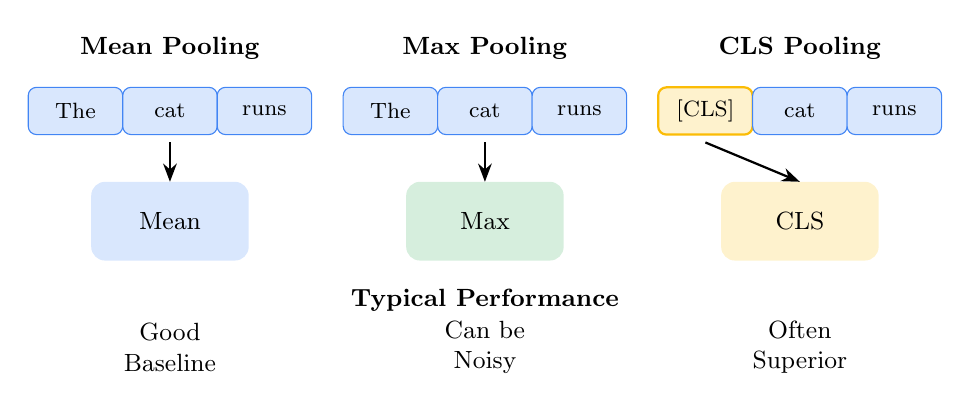
\begin{tikzpicture}[
    token/.style={rectangle, rounded corners=3pt, minimum width=1.2cm, minimum height=0.6cm, font=\footnotesize},
    clstoken/.style={token, fill=clsorange!20, draw=clsorange, thick},
    normaltoken/.style={token, fill=bertblue!20, draw=bertblue},
    pooling/.style={rectangle, rounded corners=5pt, minimum width=2cm, minimum height=1cm, font=\small},
    label/.style={font=\small}
]

% Three pooling strategies
\node[label] at (2, 6) {\textbf{Mean Pooling}};
\node[normaltoken] at (0.8, 5.2) {The};
\node[normaltoken] at (2, 5.2) {cat};
\node[normaltoken] at (3.2, 5.2) {runs};
\draw[-{Stealth}, thick] (2, 4.8) -- (2, 4.3);
\node[pooling, fill=bertblue!20] at (2, 3.8) {Mean};

\node[label] at (6, 6) {\textbf{Max Pooling}};
\node[normaltoken] at (4.8, 5.2) {The};
\node[normaltoken] at (6, 5.2) {cat};
\node[normaltoken] at (7.2, 5.2) {runs};
\draw[-{Stealth}, thick] (6, 4.8) -- (6, 4.3);
\node[pooling, fill=gptgreen!20] at (6, 3.8) {Max};

\node[label] at (10, 6) {\textbf{CLS Pooling}};
\node[clstoken] at (8.8, 5.2) {[CLS]};
\node[normaltoken] at (10, 5.2) {cat};
\node[normaltoken] at (11.2, 5.2) {runs};
\draw[-{Stealth}, thick] (8.8, 4.8) -- (10, 4.3);
\node[pooling, fill=clsorange!20] at (10, 3.8) {CLS};

% Performance comparison with qualitative labels (addressing feedback)
\node[label] at (6, 2.8) {\textbf{Typical Performance}};
\node[label, align=center] at (2, 2.2) {Good\\Baseline};
\node[label, align=center] at (6, 2.2) {Can be\\Noisy};
\node[label, align=center] at (10, 2.2) {Often\\Superior};

\end{tikzpicture}
\end{document}